\section{Adversarial Training}

The method of training used for this case follows the one proposed in the paper “I. J. Goodfellow, J. Shlens and C. Szegedy, "Explaining and harnessing adversarial examples", arXiv preprint arXiv:1412.6572, 2014”.

\begin{center}
  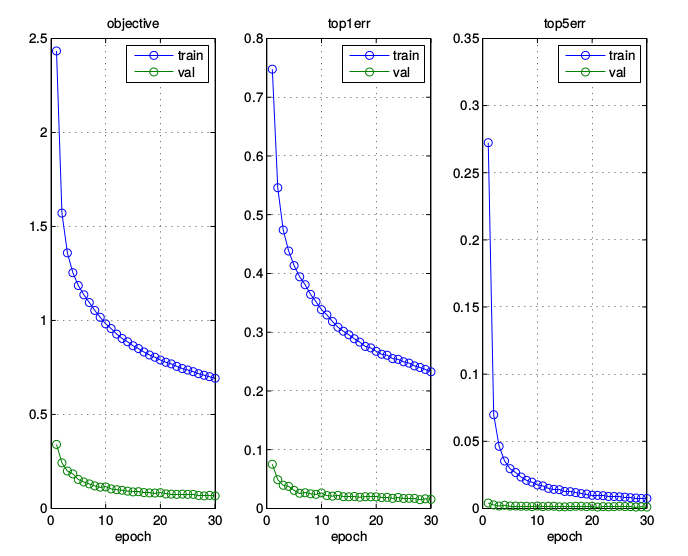
\includegraphics[width=0.7\textwidth]{img/train-adv.png}
	\label{train-mix} 
\end{center}

The objective function is modified to include adversarial examples in the training phase:

$$ 	\tilde{J}(\theta, x, y) = \alpha J(\theta, x, y) + ( 1 - \alpha)J(\theta, x + \epsilon sign(\nabla_{x}J(\theta, x, y)), y) $$

The tests were carried out as for the standard and mixed training.

\FloatBarrier
\begin{table}[h]
\centering
\begin{tabular}{@{}lll@{}}
\toprule
                               & Clean & Adversarial \\ \midrule
Correctly Predicted            & 97.97 & 77.80       \\
Error                          & 2.03  & 22.20       \\
Confidence                     & 96.03 & 79.05       \\
Confidence Correctly Predicted & 96.69 & 82.55       \\
Confidence Error               & 64.23 & 66.79       \\ \bottomrule
\end{tabular}
\caption{Test results for adversarial training model.}
\label{adv-test}
\end{table}
\FloatBarrier

As for the mixed training, the results in Table~\ref{adv-test} shows significant improvement toward the classification of adversarial examples. Compared to the standard training, the error rate dropped from ~97\% to ~22\% and the confidence for the errors also dropped significantly, from ~94\% to ~67\%.
Compared to the mixed training, the adversarial training has a lower confidence for both error and corrected prediction; it also has a higher percentage of misclassification. However, the adversarial training is faster than the mixed training.
